\documentclass[9pt]{article}

\usepackage{amsmath,amssymb}
\usepackage[utf8]{inputenc}
\usepackage{ctex}
\usepackage{epigraph}
\usepackage{amsthm}
\usepackage{multicol}

% Remove paragraph indentation for cleaner look
\setlength{\parindent}{0pt}
\setlength{\parskip}{1em}

% Reduce line spacing for more compact text
\linespread{0.2}

% Define theorem environments
\newtheorem{theorem}{Theorem}
\newtheorem{lemma}[theorem]{Lemma}
\newtheorem{corollary}[theorem]{Corollary}
\newtheorem{proposition}[theorem]{Proposition}
\newtheorem{definition}[theorem]{Definition}
\newtheorem{example}[theorem]{Example}
\newtheorem{remark}[theorem]{Remark}
\newtheorem{axiom}[theorem]{Axiom}

\renewcommand{\proofname}{Proof}


% Set CJK main font (for Chinese/Japanese/Korean characters)

% \setmainfont{Times New Roman}
\setCJKmainfont{BabelStone Han}
% doesn't work
% \setCJKmainfont{JyutcitziWithSourceHanSerifTCRegular}[
% Renderer=Basic,
% UprightFont = * ,
% FallbackFonts={BabelStone Han}
% ]



% You can also use \newfontfamily for custom non-CJK fonts if needed
% \setCJKmainfont{JyutcitziWithPMingLiURegular}[Path = ./, Extension = .ttf]
% \setCJKmainfont{JyutcitziWithSourceHanSerifTCRegular}[Path = ./, Extension = .ttf]



\newfontfamily{\jczPMingLiU}{JyutcitziWithPMingLiURegular}[Path = ./fonts/, Extension = .ttf]
% This has the best rendition for latin characters 
\newfontfamily{\jcz}{JyutcitziWithSourceHanSerifTCRegular}[Path = ./fonts/, Extension = .ttf]
\newfontfamily{\batang}{batang}[Path = ./fonts/, Extension = .ttf]
\newCJKfontfamily\koreanfont{Batang}[Path = ./fonts/, Extension = .ttf]
\newfontfamily{\taigi}{GentiumBookPlus-Regular}[Path = ./fonts/, Extension = .ttf]

% \newfontfamily{\biaoyinzi}{Biaoyinzi-2016A}[Path = ./fonts/, Extension = .ttf]

% Load ruby package for furigana (Ruby text)
\usepackage{ruby}

% IDC - ideographic description characters
% https://en.wikipedia.org/wiki/Chinese_character_description_languages#Ideographic_Description_Sequences

\newcommand{\superimpose}[2]{{%
  \ooalign{%
    \hfil$\m@th\text{#1}\@firstoftwo\text{#2}$\hfil\cr
    \hfil$\m@th\text{#1}\@secondoftwo\text{#2}$\hfil\cr
  }%
}}


% Define the \tb command

\newcommand{\tb}[2]{%
\scalebox{2}[1]{
\ooalign{%
    \hfil\raisebox{0.25em}{\text{\scalebox{0.33}{#1}}}\hfil\cr % Top text, squished and raised
    \hfil\raisebox{-0.25em}{\text{\scalebox{0.33}{#2}}}\hfil\cr % Bottom text, squished and lowered
  }%
  }
}

% The \lr command - can be combined with \tb
\newcommand{\lr}[2]{
  \scalebox{0.5}[1.0]{#1}\scalebox{0.5}[1.0]{#2}\!\!
}

% Define the \ul command for upper left positioning - for characters like 疒
\newcommand{\ul}[2]{%
  \ooalign{%
    \hfil#1\hfil\cr  % Top text (unscaled)
    \hfil\hspace{0.3em}\scalebox{0.8}{#2}\cr % Bottom text (scaled and raised)
    % \hfil\raisebox{0.2em}{\scalebox{0.5}{#2}}\hfil\cr % Bottom text (scaled and raised)
  }%
}

% Define the \tone command for upper right positioning of a diacritic
\newcommand{\tone}[2]{%
  \ooalign{%
    \hfil#1\hfil\cr  % Main text (unscaled)
    \hfil\hspace{0.9em}\raisebox{0.3em}{\scalebox{0.8}{#2}}\hfil\cr % Tone mark (scaled and raised)
  }%
}

% for vertical Chinese boxes
\usepackage{graphicx} % for \rotatebox

\newfontlanguage{Chinese}{CHN}

\setCJKfamilyfont{BabelStoneVert}[RawFeature={vertical;+vert},Script=CJK,Language=Chinese,Vertical=RotatedGlyphs]{BabelStone Han}

\newcommand*\CJKmovesymbol[1]{\raise.35em\hbox{#1}}
\newcommand*\CJKmove{\punctstyle{plain}% do not modify the spacing between punctuations
  \let\CJKsymbol\CJKmovesymbol
  \let\CJKpunctsymbol\CJKsymbol}

% Define a new environment for vertical text
\newcommand{\VertCell}[1]{\rotatebox{-90}{\CJKfamily{BabelStoneVert}\CJKmove #1}}


% *-----------------------------------------------------------------------*
% | Packages and formatting                                               |
% *-----------------------------------------------------------------------*
% *-----------------------------------------------------------------------*
% | Math & Equations     |
% *-----------------------------------------------------------------------*
\usepackage{amsmath} % For advanced math formatting
\usepackage{amssymb} % For mathematical symbols
% \usepackage{tikz} % For drawing logic decision trees


% *-----------------------------------------------------------------------*
% | Table Management                                                      |
% *-----------------------------------------------------------------------*


\usepackage{graphicx}
\usepackage{array}
\usepackage{tabularx}
\usepackage{tabularray}

\usepackage{float}      % Add the float package
\usepackage{longtable}


\usepackage[table,xcdraw]{xcolor}




% super long table

\usepackage{pdflscape} % For rotated pages

\setlength{\arrayrulewidth}{0.5mm} % Optional: to thicken table lines
\renewcommand{\arraystretch}{1.5} % Optional: to increase row height


\usepackage{makecell} 


% *-----------------------------------------------------------------------*
% | Chinese and Soochow Numerals                                          |
% *-----------------------------------------------------------------------*
% numerals.tex
% Define Chinese and Soochow numerals for chapter management

\newcommand{\soochowNumeral}[1]{%
  \ifnum#1<10
    \ifcase#1 〇\or 〡\or 〢\or 〣\or 〤\or 〥\or 〦\or 〧\or 〨\or 〩\fi%
  \else
    \ifnum#1<20
      〸\soochowUnits{\numexpr#1-10\relax}%
    \else
      \ifnum#1<30
        〹\soochowUnits{\numexpr#1-20\relax}%
      \else
        \ifnum#1<40
          〺\soochowUnits{\numexpr#1-30\relax}%
        \else
          \ifnum#1<50
            卅\soochowUnits{\numexpr#1-40\relax}%
          \else
            \ifnum#1<60
              〥十\soochowUnits{\numexpr#1-50\relax}%
            \else
              \ifnum#1<70
                〦十\soochowUnits{\numexpr#1-60\relax}%
              \else
                \ifnum#1<80
                  〧十\soochowUnits{\numexpr#1-70\relax}%
                \else
                  \ifnum#1<90
                    〨十\soochowUnits{\numexpr#1-80\relax}%
                  \else
                    \ifnum#1<100
                      〩十\soochowUnits{\numexpr#1-90\relax}%
                    \fi
                  \fi
                \fi
              \fi
            \fi
          \fi
        \fi
      \fi
    \fi
  \fi
}

\newcommand{\soochowUnits}[1]{%
  \ifnum#1=0
  \else
    \ifnum#1<4
      \ifcase#1 \or 一\or 二\or 三\fi%
    \else
      \soochowNumeral{#1}
    \fi
  \fi
}

\newcommand{\chinesenumeral}[1]{%
  \ifnum#1<10
    \ifcase#1 〇\or 一\or 二\or 三\or 四\or 五\or 六\or 七\or 八\or 九\fi%
  \else
    \ifnum#1<20
      十\chinesenumeral{\numexpr#1-10\relax}%
    \else
      \ifnum#1<30
        二十\chinesenumeral{\numexpr#1-20\relax}%
      \else
        \ifnum#1<40
          三十\chinesenumeral{\numexpr#1-30\relax}%
        \else
          \ifnum#1<50
            四十\chinesenumeral{\numexpr#1-40\relax}%
          \else
            \ifnum#1<60
              五十\chinesenumeral{\numexpr#1-50\relax}%
            \else
              \ifnum#1<70
                六十\chinesenumeral{\numexpr#1-60\relax}%
              \else
                \ifnum#1<80
                  七十\chinesenumeral{\numexpr#1-70\relax}%
                \else
                  \ifnum#1<90
                    八十\chinesenumeral{\numexpr#1-80\relax}%
                  \else
                    \ifnum#1<100
                      九十\chinesenumeral{\numexpr#1-90\relax}%
                    \fi
                  \fi
                \fi
              \fi
            \fi
          \fi
        \fi
      \fi
    \fi
  \fi
}


% *-----------------------------------------------------------------------*
% | Table of contents & Chapter management                                |
% *-----------------------------------------------------------------------*

\renewcommand{\figurename}{圗} % So figures would be labeled with 圗 instead of "figure"

% * * * Now for the table of contents
\renewcommand{\contentsname}{目錄} % Traditional Chinese characters for "Contents"
\setcounter{secnumdepth}{0} % no numbering for sections 
% Increase chapter title size in TOC
\usepackage{tocloft} % For customizing table of contents

% Redefine how chapter numbers are displayed in the TOC using Soochow numerals

% comment this out if you don't want to use the soochow numerlas
\renewcommand{\numberline}[1]{\soochowNumeral{#1}\hspace{1em}} % Use Soochow numerals for TOC chapter numbers
\makeatother


% create index - run \makeindex in the document
\usepackage{makeidx}
\makeindex



% % Custom chapter title formatting with Chinese numeral chapter numbers
\usepackage{titlesec}

% Custom chapter title formatting with Chinese numeral chapter numbers
\titleformat{\chapter}[block] % 'block' means the title appears on a new line
  {\Huge\bfseries} % Font size and bold formatting for the title
  {\soochowNumeral{\thechapter}} % Chinese character for chapter number
  {1em} % Space between the number and the title
  {\Huge} % Custom style for the chapter title itself (can modify)



% *-----------------------------------------------------------------------*
% | Document begins                                                       |
% *-----------------------------------------------------------------------*

\title{An Outline of the Siumatgwoon \\ 初論兆物觀}
\author{Hakuryo 白龍}
\date{〢〇〢〥年〢〥月〢〇日}


\begin{document}
% Avoid overfull hbox
\sloppy

% Initialize jyutcitzi processing
\jcz{}

% Generate table of contents

\maketitle


\section{Epigraphs}

\begin{table}[h]
\centering
\begin{tabular}{p{0.45\textwidth}p{0.45\textwidth}}
\epigraph{Learning the Chinese language requires bodies of iron, lungs of brass, heads of oak, hands of spring steel, eyes of eagles, hearts of apostles, memories of angels, and lives of Methuselah.}{---William Milne, who first translated the Bible into Classical Chinese in 1816.} &
\epigraph{... the Chinese [as] a people [are] characterised by a marvellous degree of imbecility, avarice, conceit and obstinacy...}{---James Matheson, cofounder of Jardine Matheson \& Co, 1840s.} \\
\vspace{1em} & \vspace{1em} \\
\epigraph{China has no philosophy, only thought.}{Jacques Derrida, 2001, Peking University.} &
\epigraph{Writing as late as 1898, Huang Qingcheng 黃慶澄 (1863--1904) placed the only Chinese monograph on logic available at the time in the category of books on ``dialects'' (fangyan 方言), that is, foreign languages, and Liang Qichao 梁啟超 (1873--1929), who was considered one of the foremost authorities in matters of new knowledge, listed the same text as a work ``impossible to classify'' (無可歸類)---alongside museum guides and cookbooks.}{---The Discovery of Chinese Logic, Joachim Kurtz}\\


% \vspace{1em} & \vspace{1em} \\
% \epigraph{Let us calculate! When controversies arise, there will be no need for dispute between two philosophers. It will suffice to take up their pens, sit down at their slates, and say to each other: Let us calculate!}{---Leibniz, *De Arte Combinatoria*, 1666} &
% \epigraph{Let us calculate! When controversies arise, there will be no need for dispute between two philosophers. It will suffice to take up their pens, sit down at their slates, and say to each other: Let us calculate!}{---Leibniz, *De Arte Combinatoria*, 1666} \\
\end{tabular}
\end{table}


\begin{table}[h]
    \centering
   
    
    \begin{tabular}{p{0.45\textwidth}p{0.45\textwidth}}
    
    \epigraph{Let us calculate! When controversies arise, there will be no need for dispute between two philosophers. It will suffice to take up their pens, sit down at their slates, and say to each other: Let us calculate!}{---Leibniz, *De Arte Combinatoria*, 1666} &
    
    \epigraph{You savages of the further seas have waxed so bold, it seems, as to defy and insult our mighty Empire. Of a truth it is high time for you to "flay the face and cleanse the heart," and to amend your ways. If you submit humbly to the Celestial dynasty and tender your allegiance, it may give you a chance to purge yourself of your past sins. But if you continue and persist in your path of obstinate delusion, your three islands will be laid waste and your people pounded into mincemeat, so soon as the armies of his Divine Majesty set foot upon your shores.}{-- Lin Zexu, the Hokkien Qing Imperialist, in Manchu occupied Canton, to HM Queen Victoria's Government, 1839} \\
    \end{tabular}
\end{table}
    
    
\section{Definitions}




\begin{definition}[Siumatgwoon]\label{def:siumatgwoon}
    A Siumatgwoon, or a Metaphysic, is a set $S$, paired with the binary relations \textit{composition} $* : S \times S \rightarrow S$ and \textit{constitution} $|:S\times S \rightarrow \{\text{True}, \text{False}\}$, such that the following axioms hold. 

    \begin{axiom}[Reflexivity]\label{ax:reflex}
    For all $a \in S$, $a|a$.
    \end{axiom}

    \begin{axiom}[Totality]\label{ax:total}
    For all $a,b\in S$, exactly one of the following holds: $a|b$ or not $a\not|b$
    \end{axiom}

    \begin{axiom}[Transitivity]\label{ax:trans}
    For all $a,b,c\in S$, $a|b$ and $b|c$ implies $a|c$.
    \end{axiom}

    \begin{axiom}[Composition Constitution]\label{ax:comp-const}
    If $a*b=c$ for some $a,b,c\in S$, then $a|c$ and $b|c$.
    \end{axiom}
\end{definition}

$a * b$ should be read is "$a$ composing with $b$", and $a | b$ should be read as "$a$ constitutes $b$". You can also read $*$ as "and", "along with", "mixed with", "reacting with", "making love with", etc. You can also read $|$ as "is a part of", "composes", "is a constituent of", "is a component of", "is a sub-object of", etc. Because we are exploring, we will enable maximal leeway in the interpretation of $*$ and $|$, and this we will see, can yield some happy and interesting structures. 

Some further clarifications: 

\begin{itemize}
\item $a\not|b$ iff $a|b = \text{false}$
\end{itemize}

The above 4 axioms are the core axioms of a Siumatgwoon. There are quite a lot of ways in which you can think about what they are. You can think of them as sure foundations you can rest upon and then launch to explore the space, or you can think of them as a set of definitions that define the metaphysics of an object, in this case a mathematical object. But all mathematical objects are metaphysical objects (though we don't know if all metaphysical objects are mathematical objects - I'd wager not - the first go-to reason one might want to appeal to is Godel's Incompleteness Theorem - I think that's the right direction but Godel won't give us the direct proof to support this intuition - it is likely going to be something beyond mathematical language. Indeed, I think there are metaphysical objects that can be described by natural language, but not mathematical language. But I digress). We can further define other types of Siumatgwoons with further axioms. A taxonomy would then emerge, defined by various properties captured by the additional axioms.

But to capture the logic inside the Sinoglyphs, which is where we are starting - and we are starting there because we believe there's an interesting logic that evolved in there - just like interesting creatures and biosphere usually evolve in isolated and unique environments. I'To specify certain more restrictive structures, we will now introduce some more axioms, that makes a siumatgwoon simple. They are "simple" because they conform to our mereological intuitions, of both the Sinoglyphs and of the world.

\begin{definition}[Simple Siumatgwoon]\label{def:simple}
A Simple Siumatgwoon $S$ is a siumatgwoon where:
\begin{axiom}[Antisymmetry]\label{ax:antisymmetry}
    For all $a,b\in S$, if $a|b$ and $b|a$ then $a=b$.
\end{axiom}
\begin{axiom}[Finite composition]\label{ax:finite_composition} 
    Every object is finitely composed. For any $x\in S$, $x = y_1 * y_2 * y_3 \cdots y_n$ for some finite number $n$.
    In other words, there is no object that is composed of infinitely many objects.
\end{axiom}
    
\begin{axiom}[Finite Constitution]\label{ax:finite_constitution} 
For any $x \in S$, there are only finitely many objects $y_1, y_2, \ldots, y_n \in S$ such that $y_1, y_2, \ldots, y_n | x$.
\end{axiom}

\begin{axiom}[Unique Decomposition]\label{ax:unique-decomposition} 
    For any $x\in S$, the longest decomposition into objects of $S$ is unique. We can speak of the longest decomposition of an object, because we have axiom \ref{ax:finite_composition}, which says that every object is finitely composed.
\end{axiom}
\end{definition}

\ref{ax:antisymmetry} says no two distinct objects constitute each other. It rules out circular identity via mutual constitution. So you can't have chains like atoms|humans|universe|atoms - no embedded universes in atoms like in \ruby{手塚 治虫}{おさむ てずか}'s 《\ruby{火の鳥}{ひのとり}》 

\ref{ax:finite_composition} is a cardinality constraint on the composition operator $*$. Antisymmetry is a constraint on the constitution relation $|$. There's no logical connection between a limit on the number of components in a composition and antisymmetry.

Note that antisymmetry says nothing about how many objects compose another—only about how $|$ relates distinct objects. You could easily construct a model where antisymmetry holds, but some elements are infinitely composed (e.g., think of $x = a_1 * a_2 * a_3 * \cdots$ in a naïvely defined algebra).

One should also note that Axiom \ref{ax:antisymmetry} antisymmetry also rules out the possibility of a simple siumatgwoon modeling objects that obey sentences like "man is a part of nature, and nature is a part of man" or "the Tao is part of everything, and everything is part of the Tao" - as clearly the philosophies or metaphysics of those two utterances do not admit that just because $\text{man} | \text{nature}$ and $\text{nature} | \text{man}$, then $\text{man} = \text{nature}$, or that $\text{Tao} | \text{everything}$ and $\text{everything} | \text{Tao}$, then $\text{Tao} = \text{everything}$. 


Axiom \ref{ax:finite_constitution}, finite constitution, is a cardinality constraint on the constitution relation $|$. The point of both \ref{ax:finite_composition} and \ref{ax:finite_constitution} is to ground us in the world of finite compositions and finite constitutions. 

It says you cannot make a superobject by composing infinitely many objects - composition is finite. Obviously, one can eventually relax this and figure out how things will look. Those sensitive to theological arguements might already detect that finite composition precludes the existence of 㕦 in a Siumatgwoon so defined. If God is infiniite in the sense it has infinitely many attributes, then it is not possible to model God in a simple siumatgwoon. However, it seems perfectly intuitive to argue that all things have infinitely many attributes, so nothing can actually be modeled by a simple siumatgwoon. Perhaps a fruitful way to then model these objects of infinite attributes, is not to relax the axiom, but to consider a sequence of simple siumatgwoons $\text{兆}_0,\text{兆}_1, \text{兆}_2, \text{兆}_3, \ldots$, that somehow converge, where the limiting object is indeed an object of infinite attributes. Obviously, to define some kind of limiting mechanism or concept of converge, you'd need to have some concept of open sets, or stronger still, a metric. Let's not get into that. 

% Suppose we want to model the Thames, $\text{河}_{\text{Thames}}$, and in $\text{兆}_0$, we have 
% $$\text{兆}_0 = \{\text{河}, \text{河}_{\text{Thames}}\}$$
% $$\text{兆}_1 = \{\text{河}, \text{河}_{\text{Thames}}\}$$
% In $\text{兆}_0$

It will be very interesting to see what kind of objects will be yielded if we relax these two axioms - to infinite compositions and infinite constitutions. How will they look like?

Well, if we relax \ref{ax:finite_constitution}, one can have a siumatgwoon $S$ where everything can be infinitely decomposed. So there are no atoms - everything can be cut smaller and smaller and smaller - without end.

This is also a cardinality restriction—this time on the domain of constitutors of any object. Antisymmetry only constrains symmetric pairs in $|$, not how many $y$'s can point to $x$.

A model could satisfy antisymmetry yet have an object $x$ with infinitely many distinct constituents $y_i$ such that $y_i|x$, without any pair $y_i, y_j$ satisfying $y_i|y_j \wedge y_j|y_i$.

The uniqueness decomposition axiom, axiom \ref{ax:unique-decomposition}, is a uniqueness constraint on the decomposition of an object into its constituents. It says that the longest decomposition of an object is unique. It says that nothing can made of up of two sets of objects. If you have two different sets of components, then it's not possible to make the same thing. It says: among all decompositions of $x$, there is a unique one of maximal length (i.e. atomic resolution). This requires some structural property of $*$, perhaps associativity or atomic irreducibility. 

Antisymmetry doesn't regulate the structure of compositions—just the equality condition under mutual constitution. Even with antisymmetry, multiple maximal-length decompositions could exist, e.g., due to commutativity or ambiguity in decomposition paths, unless you restrict the structure of $*$.



These are some really weird objects indeed. But they are definitely not anything like the Sinoglyphs - at least not right now. 




Does the size of the infinity make things even more interesting? Careful now, we are trying to do what Leibniz didn't do, not to roleplay Cantor. 

Before we discuss some firther definitions, of Elementals, Generators, Atomics, let us remark some pattens we see in the Sinoglyphs. 

The first thing to remark is that Westerners have translated the 邊旁 into "radicals" - as if they're solutions to a quadratic equation, which means then they thought the whole sinoglyph itself is like an equation to be solved. 

If we take these radicals, that compose a sinoglyph, we'd say that they are the elementals of the sinoglyph. 

The way I came up with the set of definitions for atoics, elementals, generators - was to model the Sinoglyph writing system. Oftentimes, in the Sinoglyph system, as it appears to us, all three sets are the same. 

But if we consider a possible extension to the Chinese Character writing system, and simply consider the idealised and fully evolutionarily searched space of possible evolutionary trajectories of the Chinese character writing system, we can arrive at an idealised symbol combination system - that's the Sinoglyph. That Sinoglyph symbol manipulation system, has a structure. And that structure is its Siumatgwoon. And we are now trying to model that structure with some axioms. 

Atomics are basically 獨體字. They stand alone. They cannot be decomposed, and nothing constitutes them besides themselves.

Elementals are basically any sinolgyph that cannot be fully decomposed. Something else might constitute it, but its constitutes can be composed to make the whole the elemental. There's something more in the elemental than just whatever constituting. An elemental might have many many constituents, but the elemental is somehow larger than the composition of its parts. This can be called emergence. 

But not all elementals exhibit emergence. Because all atomics are elementals. Since atomics are constituted by themselves, and the atomic needs nothing to be composed with to be itself, atomics are elementals with no emergence. 


The elementals largely correspond to the kind of compound sinoglyphs 合體字 that are called phonosemanophores - 形聲字。 

Now let's think about how a 形聲字 works. Let's take the classic example of 江河, specifically 河. The Chinese character 河 is a 形聲字. 
$$\text{河}$$
It is composed of 氵(water) and 可 (ho). Ho is just a name. You might as well right it like this $$\text{氵}_{\text{可}}$$. But the sound is immaterial, it's just an index. It might as well be $a,b,c$

$$\text{氵}_{a},\text{氵}_b,\text{氵}_c$$
But the important thing is that picks something out. It picks out from the set of all objects that are constituted by water the thing that is "river". You might as very well write it as $$\text{氵}_{river}$$. 

The Chinese way of writing "river" is not different from writing it as "氵river". It says that "river" belongs to the class of things that are constituted of "氵"(water); it says "river" is a "氵" thing; it says "river" belongs to the set, the class, the category of "氵" things; but most importantly, it says: I don't know how "river" is composed, but I do know it is constituted of "氵". So there's something beyond water that makes a river - but I don't know what all the stuff that composes a river is, or hanc marginis exiguitas non caperet.

What this immediately suggest is a 系 system. A 金木水火土系 system. A system where elementals can be long to 金系, 木系, 水系, 火系 土系 system is a Siumatgwoon, where each 系 contains (but is not limited to) elementals that are constituted of the well, the "Head" of the 系. So the head, of a 土系 is 土. The head of a 金系 is 金. The head of a 木系 is 木. The head of a 水系 is 水. The head of a 火系 is 火. 

We want to capture this - the set of all objects exhibiting emergence from a certain "head". Let us call this set of head x the x-系. 



\begin{definition}[系 (Hai) Elements]\label{def:hai-elements}
    The set x-系, written as $\langle x \rangle$ is defined to be 
    
    $$\langle x \rangle := \{ s\in S: x|s \text{ but } \not \exists y_1, y_2,\ldots, y_n \in S \text{ such that } s=x*y_1*y_2*\cdots*y_n\}$$. 
    \end{definition}

    x-系 elements roughly correspond to the 形聲字 in Chinese characters - if you do not consider the phonetic component of a character to be full elements inside the Siumatgwun but mere indices. In other words, one does not view 江、河、湖、海 as 水工、水可、水胡、水每 but as $\text{水}_\text{工}、\text{水}_\text{可}、\text{水}_\text{胡}、\text{水}_\text{每}$. In this sense, one can see there is no element $y \in S$ such that $\text{水}y=\text{水}_\text{工}=\text{江}$.
    
    
    Let us now take this definition and apply it to entire sets. 
    
    \begin{definition}[X-系]\label{def:hais-of-sets}
        Let $X\subseteq S$. The $X$-系 is defined to be $\langle X \rangle := \cup_{x\in X} \langle x \rangle$.
    \end{definition}
    
Being elementals, they cannot be fully decomposed. So what's in an x-系?Say, 木系 $\langle \text{木} \rangle$?

Well, it contains $\text{木}$, because $\text{木}$ is cannot be further decomposed. But we also have the other trees, 松,柏,柳,桃,梅, so we can say 

$$\text{木}_{\text{公}},\text{木}_{\text{白}},\text{木}_{\text{卯}},\text{木}_{\text{兆}},\text{木}_{\text{每}},  \text{木} \in \langle \text{木} \rangle$$



But note that $\text{林}, \text{森},  \text{焚} \not\in \langle \text{木} \rangle$

Does the head of a 系 have to be an atomic element? No, not at all! In fact, the head of a 系 could itself be an elemental like 河, or a proper compound like 雲. Consider the siumatgwoon $S = \{\text{雨}, \text{云}, \text{雲}, \text{霒}, \text{霕}, \text{霴}, \text{靉}\}$. In this set clearly the atoms are $\{\text{雨}, \text{云}\}$, but the elementals are $\{\text{雨}, \text{云}, \text{霒}, \text{霕}, \text{霴}, \text{靉}\}$. So $\{\text{霒}, \text{霕}, \text{霴}, \text{靉}\}$ are all in $\langle \text{雨} \rangle$ and in $\langle \text{云} \rangle$ and also in $\langle \text{雲} \rangle$.

But there's no reason why elementals, 形聲字, themselves, cannot be the head of a 系. Why shouldn't there be say an object $x=\text{河}_{a}$ or $river_{a}$ that we know is a kind of river, but we don't know what all the other constituents are to make it more than just a "typical"river? I mean, it's pretty obvious that The Thames, La Seine, The Hudson, The Jyugong, are all rivers, i.e.: 
$$\text{河} | Thames, Seine, Hudson, \text{珠江}$$

Which is to say 
$$\text{河} |  \text{河}_{Thames},\text{河}_{Seine},\text{河}_{Hudson},\text{河}_{\text{珠江}} $$
but we can't write down all the other constituents that make them more than just a river, and not how they differ from each other either. So, 
i.e.: 
$$\text{河}_{Thames},\text{河}_{Seine},\text{河}_{Hudson},\text{河}_{\text{珠江}} \in \langle \text{河} \rangle$$



Let us now get some proper definitions.


\begin{definition}[Atomics]\label{def:atomics}
    An element $a \in S$ is atomic if for all $x\in S$, if $x|a$ implies $x=a$, i.e. $a$ is atomic iff only anything that constitutes $a$ is $a$ itself.
\end{definition}

\begin{definition}[Elementals]\label{def:elementals}
    An element $e \in S$ is elemental if and only if for all $x_1, x_2, x_3, \ldots, x_n \in S$ where $x_1, x_2, x_3, \ldots, x_n | e$, we have cannot find a finite sequence drawn from $x_1, x_2, x_3,\ldots, x_n $ such that it composes $e$. In other words, an elemental has no non-trivial decomposition other than $e = e$. 
\end{definition}


Note that Siumatgwoons do not swear alliegance to commutativity or associativity. $a*b$ might not equal to $b*a$ and $a*(b*c)$ might not equal to $(a*b)*c$. Both sucrose and fructose have the same molecular formula of $\text{C}_6\text{H}_{12}\text{O}_6$, and so $\text{C}, \text{H}, \text{O} | sucrose, fructose$, but sucrose and fructose are not the same object. Listing the constituents of an object also does not specify how those individual constituents are themselves composed to form components that form the object, which means we don't actually know how many times $C, H, O$ appear in sucrose or fructose. The point of the definition of the elemental, is to say, no matter how you arrange the constituents, no matter how many times each of the constituents appear in a composition, you cannot compose the object from those constituents alone. Again, emergence is at play here.



We quickly define the sets of atomics $A$ and the set of elementals $E$.

\begin{definition}[Atomic Set]\label{def:atomic-set}
    The set $S_A \subseteq S$ is called the atomic set of $S$. It is the set of all atomic elements inside $S$.
\end{definition}

\begin{definition}[Elemental Set]\label{def:elemental-set}
    The set $S_E \subseteq S$ is called the elemental set of $S$. It is the set of all elemental elements inside $S$.
\end{definition}


\begin{lemma}[Atomics are Elementals in Simple Siumatgwoons]\label{def:atomics-are-elementals-in-simple-siumatgwoons}
    All atomics are elementals in simple siumatgwoons. For all simple siumatgwoons $S$, $A \subseteq E$.
\end{lemma}
\begin{proof}
    Let $a \in A$. $a$ clearly constitutes itself, so $a=a$. If $a$ is not an elemental, then there exists a decomposition $a=b*c$ for some $b,c \in S$. By atomicity, $b=a$ or $c=a$. But then we can apply the same argument again, so $a=a*a$. And we can go ad infinitum, so $a=a*a*\cdots$. But this contradicts \ref{ax:finite_composition}, which states every object in a simple siumatgwoon are composed by a finite number of objects. Therefore, $a$ cannot have any decomposition other than $a$. Therefore, $a$ is an elemental.
\end{proof}


\begin{lemma}[Atomics]\label{def:atomics}
    The decomposition of an atomic in a simple Siumatgwoon is unique. i.e. $a=a$ is the only decomposition of an atomic.
\end{lemma}
\begin{proof}
    As proven above.
\end{proof}



\begin{definition}[Generators]\label{def:generators}
    A set $G \subseteq S$ is a generator of $S$ if and only if every object $x \in S$ can be expressed as a composition (trivial or compound) of objects from $G$.
\end{definition}

\begin{theorem}[Generator sets exist in simple siumatgwoons]\label{thm:generator-sets-exist-in-simple-siumatgwoons}
    In a simple siumatgwoon, there exists a non-empty subset $G_{S} \subseteq S$ such that every element $x \in S$ is a product of a finite sequence of elements from $G_S$, i.e., $x = g_1 * g_2 * \cdots * g_n$, where $g_1, \dots, g_n \in G_S$.
\end{theorem}

\begin{proof}
    This is clearly true, because any object $x\in S$ is always a finite composition of itself. So we can just let $G_S = S$. In other words, the set of all objects in $S$ is a generator set of $S$.
\end{proof}

\begin{lemma}[Elementals are in every generator set]\label{lem:elementals-are-in-every-generator-set}
    In a simple siumatgwoon, $E\subseteq G$ for any generator set $G$.
\end{lemma}
\begin{proof}
    Since any generator set $G$ must generate all objects in $S$, the generator set $G$ must generate all elementals in $E$. But elementals have non-trivial decompositions, so they are generated only by themselves. Therefore, to generate the elementals, the generator set $G$ must contain all elementals. Therefore $E\subseteq G$. This also means no generator set can be smaller than $E$.
\end{proof}

\begin{lemma}[All objects are either elementals or compounds]\label{lem:elementals-are-not-compounds}
    For any $x\in S$, $x$ is either an elemental or a compound.
\end{lemma}
\begin{proof}
    If $x$ is an elemental, then it is an elemental. If $x$ is not an elemental, then it has a non-trivial decomposition. Then it is a compound.
\end{proof}

\begin{lemma}[Compounds are composed by elementals]\label{lem:compounds-are-composed-by-elementals}
    If an object $x\in S$ is a compound, then it is composed by elementals.
\end{lemma}
\begin{proof}

    If $x$ is a compound that cannot be decomposed into only elementals, then in any decomposition of $x$ you can always find a compound $c_1$ in the decomposition. Because $c_1$ is a compound, it can also be decomposed, and in any decomposition of $c_1$ you must always be able to find a compound $c_2$ in the decomposition, because if otherwise, $c_1$ will be composed entirely of elementals, and so will $x$. But the argument applies for $c_2$ as well, and you will be able to find a compound $c_3$. This can be done indefinitely and you will get a sequence of $c_1, c_2, c_3, \ldots$, and by their nature, we have  $\ldots, c_1|c_2|c_3|\cdots|x$, and they are all distinct. This means, for $x$, we can find a infinite set of $c_1, c_2, c_3, \ldots$, all constitutents of $x$. But this is in violation of axiom \ref{ax:finite_constitution}, the finiteness of constitution. Therefore, by contradiction, there can be no compound that is composed of only compounds - therefore, all compounds are composed of elementals.
\end{proof}


Note that in a non-simple siumatgwoon where compositions can go on definitely deep, you can always chop at some level, and whatever higher than the level chopped will yield a simple siumatgwoon - because that seems to be our universe. 


Now we move to a stronger theorem.

\begin{theorem}[The elementals are a generator set in simple siumatgwoons]\label{thm:elementals-are-a-generator-set-in-simple-siumatgwoons} 
    In a simple siumatgwoon, the set of elementals $E$ is a generator set of $S$.
\end{theorem}

\begin{proof}
    We have proven $E\subseteq G$ for all generator sets $G$ in $S$. Now we need to prove that for any $x\in S$, $x = e_1 * e_2 * \cdots * e_n$ for some $e_1, \dots, e_n \in E$.

    From \ref{lem:compounds-are-composed-by-elementals}, we know that any compound $x$ is composed by elementals. So we can write $x = e_1 * e_2 * \cdots * e_n$ for some $e_1, \dots, e_n \in E$.

    But since every element in $S$ is either an elemental or a compound, and compounds are all composed by elementals, any element in $S$ is therefore a composition of elementals - in other words, generated by the elementals. Therefore $E$ is a generator set of $S$.
\end{proof}


Now we put it all together.
\begin{theorem}
    Let $S$ be a Simple Siumatgwoon. And let $E$ be the set of elementals of $S$. Then: 
    \begin{enumerate}
        \item $E$ is a generating set, and 
        \item The decompositions into elementals are unique.
    \end{enumerate}
\end{theorem}
\begin{proof}
    We have already proven (1) in \ref{thm:elementals-are-a-generator-set-in-simple-siumatgwoons}. Now we need to prove that the decompositions into elementals are unique.

    In a simple siumatgwoon, the longest decomposition is unique. Now since every object in a simple siumatgwoon is a composition of elementals, and since elementals cannot be further decomposed, the decomposition of that object into elementals is the longest decomposition. Therefore, the decomposition of any object into elementals is unique.
\end{proof}


Now we let us return to x-系 sets.

Then we can prove the following lemma. 
\begin{lemma}[The emergence of a constituted is emergence of the constituent]\label{lem:emergence-of-a-constituted-is-emergence-of-the-constituent}
    If $a|b$, then $ \langle b \rangle \subseteq \langle a \rangle$.
\end{lemma}
\begin{proof}
    If $a|b$, then for any $x\in \langle b \rangle$, because $a|b$ and $b|x$, we have $a|x$. And since $x$ is an elemental, it has no non-trivial decomposition. An object constituted by $a$ and has no non-trivial decomposition is an $a$-系 object, so $x \in \langle a \rangle$. Therefore, $\langle b \rangle \subseteq \langle a \rangle$
\end{proof}

We clearly see this. $
\langle \text{水}_\text{工} \rangle = \langle \text{江} \rangle \subseteq
\langle \text{水} \rangle$. 

Indeed,$\langle \text{靉} \rangle, \langle \text{霴} \rangle, \langle \text{霕} \rangle, \langle \text{霒} \rangle \subseteq \langle \text{雲} \rangle \subseteq \langle \text{雨} \rangle$

Or to take more interesting example, if we take $\text{江湖}$ is an object itself of itself, then the set $\langle \text{江湖} \rangle = \{\text{江湖}_{1}, \text{江湖}_{2}, \ldots\}$ obeys the following 


$\langle \text{江湖} \rangle \subseteq \langle \text{江} \rangle,  \langle \text{湖} \rangle \subseteq \langle \text{水} \rangle$

\begin{lemma}[Every elemental has an atomic constitutent]\label{lem:every-elemental-has-an-atomic-constituent}
    Every elemental $e$ has an atomic constituent $a$ such that $e|a$. In other words, for any $e \in E$, there exists an $a \in A$ such that $e \in \langle a \rangle$.
\end{lemma}
\begin{proof}
    Assume for contradiction that $e$ has no atomic constituents. 

    Then we know that there must be an $x$ such that $x$ is a constituent of $e$, and that $x\neq e$, because if for all $x$ such that $x|e$, $x=e$, then $e$ is atomic. 

    So let us assume there is an $x$ such that $x|e$ and $x\neq e$. $x$ is either an elemental or a compound. We know all compounds are composed of elementals. So, regardless of whether $x$ is an elemental or a compound, there is going to be an elemental $f_1$ such that $f_1|x$. Per assumption, this elemental $f_1$ must not be an atomic, so another elemental $f_2\neq f_1$ such that $f_2|f_1$. But the argument can be applied again, indefinitely. But this means, we obtain an infinite set of $f_1, f_2, \ldots$ such that $f_i|f_{i+1}$ for all $i$. But this contradicts \ref{ax:finite_constitution}, which states every object in a simple siumatgwoon are composed by a finite number of objects. Therefore, every elemental has an atomic constituent.
\end{proof}









This also implies, the following theorem. 
\begin{theorem}[Every 系 set is a subset of a 系 set whose head is atomic]\label{thm:every-hai-set-is-a-subset-of-a-hai-set-whose-head-is-atomic}
    For any $x\in S$, $\langle x \rangle \subseteq \langle a \rangle$ for some $a\in A$.
\end{theorem}
\begin{proof}
    Consider $\langle x \rangle$. $x$ is either an elemental or a compound. And every compound is made of elementals. So there exists an elemental $e$ such that $e|x$. Therefore $\langle x \rangle \subseteq \langle e \rangle$. 
    
    By \ref{lem:every-elemental-has-an-atomic-constituent}, we know that for any $e \in E$, there exists an $a \in A$ such that $a|e$, so we have $\langle e \rangle \subseteq \langle a \rangle$. Therefore, there is an atomic $a$ such that $\langle x \rangle \subseteq \langle a \rangle$
    
\end{proof}


Can we prove in a simple siumatgwoon?

Now we can prove something even more interesting. 
\begin{theorem}[$\langle A \rangle = E$ in simple siumatgwoons]\label{thm:hais-of-sets-are-siumatgwoons}
    In a simple siumatgwoon, $\langle A \rangle = E$ for any $A\subseteq S$.
\end{theorem}
\begin{proof}
    We will first prove that $\langle A \rangle \subseteq E$, and then we will prove that $E \subseteq \langle A \rangle$.

    Let us prove that $\langle A \rangle \subseteq E$.  


 
\end{proof}

\subsection{Examples of Siumatgwoons}

What are some examples of Siumatgwoons? 



\subsubsection{The Chinese Characters, 字}

The Chinese characters, which inspired this whole mathematical exercise, is clearly a Siumatgwoon. If we exercise the synonym exchange of "Siumatgwoon" with "Metaphysic", then to say the Chinese characters are a siumatgwoon, then this is to say that the Chinese characters is a Metaphysic. 

Unfortunately we can't really \textit{prove} that the Chinese characters are indeed a siumatgwoon, given there's an infinite number of them, and we do not have a generating rule for all Chinese characters. 

However, if given any random subset of all Chinese characters, we can prove that it is a siumatgwoon. 

Let's consider one example. Let's consider the subset of Chinese characters that are composed of only 1 stroke. Consider the following set of Chinese characters: 

$$S=\{\text{日},\text{月}  ,\text{皿},\text{明},\text{盟},\text{盥}\}$$

Let us first verify that this is indeed a siumatgwoon. But here's now an interesting question, how are $*$ and $|$ defined? Well, intuitively, we can say a Chinese character $c = a *b$ if $c$ is made of $a$ and $b$. And we can say that $c|a$ if $c$ appears in the character $a$. Not terribly helpful or illuminating, perhaps - but is this any less illuminating than defining the valuation of $\phi \wedge \psi$ to be the "$0$ unless both the valuation of $\phi$ and the valuation of $\psi$ are $1$"? Tautology is where judgement, human intuition, and the exercise of the human choice to grant admission works, and must work - for logic and mathematics to start. 

One might note there's something seemingly inherently linked to the behaviour of substrings here. If the logic of a siumatgwoon is merely a logic for substrings, which would be plausible since the project of the siumatgwoon appears to be fundemntally a merelogical project, then we might have been rather inflating the intellectual importance of the siumatgwoon. I shall sincerely pray this to not be the case; and I also don't believe this is the case.

So does $S$ satisfy the axioms of a siumatgwoon? 

Axiom \ref{ax:reflexive} says any $s\in S$ satisfies $s|s$. This is clearly true. 
Axiom \ref{ax:total} is clearly true as well. Since there is no character which is simultaneously constituted by two different sets of characters in $S$.

Axiom \ref{ax:transitive} says that for any $s_1, s_2, s_3 \in S$, if $s_1|s_2$ and $s_2|s_3$ then $s_1|s_3$. This is vacuously true, because ha! There are no such three characters in $S$! 

Axiom \ref{ax:composition} says that for any $s_1, s_2 \in S$, $s_1*s_2 \in S$. This is also clearly true - by definition of $*$ and $|$.

So in this very boring example where all 4 axioms are trivially or vacuously true, let us now ask about its atomic set $A$, its elemental set $E$.

Now clearly, we have 
$$A=E=\{\text{日},\text{月},\text{皿}\}$$

So indeed $A\subseteq E$. And indeed in this case, $A=E$, because there are no emergent elements. There are no 系 sets with more than one object - all emergent sets are singletons. This is immediately visible by the fact there are no phonosemanophores 形聲字. And indeed, as proven before, the smallest generator set is indeed $E$, as every object of $S$ is composed by $E$.

And the set of compounds $\{\text{明},\text{盟},\text{盥}\}$ is clearly disjoint from the set of elementals $\{\text{日},\text{月},\text{皿}\}$. 

It is also immediately obvious, that $S$ is a simple siumatgwoon, because no character in $S$ is composed of or constituted by infinitely many other characters in $E$. And clearly, each character is uniquely composed by the elementals, as we can see from the compounds: $\text{盟} =\text{明}*\text{皿} = \text{日}*\text{月}*\text{皿}$.


At this point, it might be really tempting to say if a siumatgwoon is finite, it must be a simple siumatgwoon. But alas, no. We will see this later.


Consider the following siumatgwoon: 
$$S=\{\text{骨}, \text{身}, \text{人}, \text{本}, \text{體}, \text{骵}, \text{躰}, \text{体}\}$$

Let us skip the verification of the axioms, and get to the interesting stuff.

Here, we have 
$$A=\{\text{骨}, \text{身}, \text{人}, \text{本}\}$$
and 
$$E=\{\text{骨}, \text{身}, \text{人}, \text{本}\, text{體}\}$$.


So here, $A\neq E$, because there are emergent elements - phonosemanophores 形聲字. 

What we should immediately point out here is that to the seasoned sinoglyph scholar, he will immediately recognize that 體, 骵,躰,体 are all variants of the same "character", the same "glyph", the same "sign". They point to the same thing. They are \ruby{異體字}{いたいじ}. It is therefore very tempting to then write that the "true form" of $S$ is actually this:



$$S=\{\text{骨}, \text{身}, \text{人}, \text{本}, \text{體} = \text{骵} = \text{躰} = \text{体}\}$$.

Now, if this makes any sense, then we can immediately see that this is not a simple siumatgwoon, because there is a compound with two different decompositions: 


\begin{align}
    \text{體} &= \text{骵} = \text{骨} * \text{身} \\
             &= \text{躰} = \text{身} * \text{本} \\
             &= \text{体} = \text{人} * \text{本}
\end{align}
    
It is still a siumatgwoon. But it is not a simple siumatgwoon. 

One should note that there is something very degenerate in imposing the equality $\text{體} = \text{骵} = \text{躰} = \text{体}$. 

On intuitive and philosophical level, it is not appropriate to write that $\text{體} = \text{骵} = \text{躰} = \text{体}$. The most naive argument is probably that the 4 different glyphs are not really saying the same thing. We are not here to do psychology, but one should consider the psychological and performative motivation behind when one writes $\text{骵}$ instead of $\text{體}$. One is making the point that the referent of $\text{體}$ can actually be decomposed into $\text{骨}$ and $\text{本}$ - that while one party believes $\text{體}$ is an emergent object, the other party believes that $\text{體}$ is actually completely composed by $\text{骨}$ and $\text{本}$ ("a body 體 or 骵 is the basis 本 of a bone 骨" - or some other imaginative formulae involving the 骨 and 本). So in this argument, the two assertions carry different ontological commitments on the nature of what a body is. So $\text{體} \neq \text{骵}$.

This is an interesting argument, but the argument allowing for $\text{體} \neq \text{骵}$ is really intuitively compelling. Obviously, when the champion of the variant writes $\text{骵}$ instead of $\text{體}$ wherever $\text{體}$ appears, say in $\text{身骵}$,$\text{個骵}$,$\text{本骵}$,$\text{人骵}$,$\text{國骵}$,$\text{聖骵}$,$\text{靈骵}$,$\text{天骵}$,$\text{物骵}$, he is clearly making the point that the referent of $\text{體}$ is actually composed by $\text{骨}$ and $\text{本}$. In other words, the referent of $\text{體}$ is the same as the referent of $\text{骵}$. So $\text{體} = \text{骵}$. 

There's also an aesthetic reason why we would be tempted by allowing for $\text{體} = \text{骵} = \text{躰} = \text{体}$, as it seems to allow us this kind of derivation: 

\begin{align}
    \text{骨}, \text{本} &| \text{骵}, \\
    \text{身}, \text{本} &| \text{躰}, \\
    \text{人}, \text{本} &| \text{体}, \\       
    \text{骵} = \text{體} &= \text{躰} = \text{体} \\
    \therefore \text{骨}, \text{人}, \text{本}, \text{身} &| \text{骵}, \text{躰}, \text{体}, \text{體} 
\end{align}

Well the conclusion that "bone", "man", "base", "body", are all constituents of "body" is very intuitively compelling. It's not yet certain what the rules of reference are employed here, but whatever they are, if this derivation is admitted, then we can then work to formalize those rules of reference, and the logical structure of the mathematical object of Siumatgwoon would be richer for it. 

But this introduces some very degenerate behaviiour into the Siumatgwoon object. The genie responsible is the $=$ relationship. It breaks our semantic definition of $*$ and $|$, as $*$ and $|$ are no longer matters of considering what the substrings of a Chinese character is, because a character like $\text{體}$ can now have "hidden" constituents $ \text{人}, \text{本}, \text{身}$. 

Also, to allow for $=$ in a siumatgwoon, it might introduce certain undesirable set theoretic behaviour. Not quite sure how to demonstrate this, but the potential for violation is intuitively plausible. Notationally, if we allow for $=$, in set theoretic language, the objects $\text{體}, \text{骵}, \text{躰}, \text{体}$ are all just the same object. So notationally, 

$$S=\{\text{骨}, \text{身}, \text{人}, \text{本}, \text{體} = \text{骵} = \text{躰} = \text{体}\}$$.

is the same as 
$$S=\{\text{骨}, \text{身}, \text{人}, \text{本}, \text{體}\}$$.

But that's most definitely not what we want to say. And saying that seriously simplifies the structure that one is trying to describe, however naively.

What one is trying to say, is that there is an object $S$ such that 

$$S=\{\text{骨}, \text{身}, \text{人}, \text{本}, \text{體} , \text{骵}, \text{躰}, \text{体}\}$$.

but the objects $\text{體} , \text{骵}, \text{躰}, \text{体}$ are "identical", "equivalent", in some sense, up to some kind of relation - are variants of the same thing. Given the use of "identical", "equivalent", and the very symbol $=$, it seems very compelling that these objects are related by an equivalence relation - reflexivity, symmetry, and transitivity being the core properties governing them. We shall call their relation "synonymy", represented by the symbol $\sim$. So we can write this instead: 

$$S=\{\text{骨}, \text{身}, \text{人}, \text{本}, \text{體} ~ \text{骵} ~\text{躰} ~\text{体}\}$$.

And so the set theoretic collapse vis-a-vis $=$is avoided. 

The synonymy relation $~$ will open up significant structures of interest for us to explore, which we will do later.

Now, we must ask the question, are there other siumatgwoons aside from the Chinese characters? Why yes, of course. 



\subsubsection{The Roman Numerals $\mathfrak{R}$}

One can clearly see that Roman Numerals $\mathfrak{R}$ are a Siumatgwoon. However, to appreciate the characteristics that make it a Siumatgwoon, let us consider the subset of Roman Numerals from 1 to 10, which we shall show to also be a Siumatgwoon.

$\mathfrak{R}_{1,10} = \{I, II, III, IV, V, VI, VII, VIII, IX, X\}$

We will say that for two elements $a,b \in \mathfrak{R}_{1,10}$, $a|b$ iff the glyph $a$ appears in $b$. As such, we can say $I | II$ and $I|III$ as an example, and that $V|IV$ and $X|IX$. 

For any elements $a,b\in \mathfrak{R}_{1,10}$, if the glyphs $ab$ so written together forms a glyph that also appears in $\mathfrak{R}_{1,10}$, then we'd say that $a*b\in \mathfrak{R}$.

Now, it's clear that Ax 1 is satisfied trivially. 

Ax 2 is also satisfied trivially.

Ax 3 is also satisfied. 

Ax 4 is also satisfied. As an example: $I | III, III | VIII$ and we have $I|VIII$.

So therefore, $\mathfrak{R}_{1,10}$ is a Siumatgwoon. 

It is also interesting to note that as per the definition of $\mathfrak{R}_{1,10}$, it is not compositionally closed. For example, $II * III$ is not in $\mathfrak{R}_{1,10}$. This makes the Siumatgwoon different from a group, where all compositions are contained inside the group. Intuitively, perhaps this suggests the Siumatgwoon is less rich in structure than the mathematical group? Also, note that what $II * III$ should be in $\mathfrak{R}_{1,10}$ is represented by $V$. Intuitively, we can feel that in some sense, $II * III = V$ - that they're synonymous, identical, referring to the same referent. This is not unlike the presence of variant characters in the Sinoglyphs, such as 體 (body, object)=骵=躰=体, or信 (trust) = 𬢭 = 伩 = 訫 = 㐰… Intuition should hint that this will yield some interesting structures if we pursue the investigation down this path.

\subsubsection{Any Numerals System}

The fact that the Roman Numerals are a Siumatgwoon should intuitively suggest that any numeral system is a Siumatgwoon. In fact, let us consider the world's many numeral systems, and see if there is one where it is not a siumatgwoon. 

\begin{center}
\begin{tabular}{|l|c|c|c|c|c|c|c|c|c|c|}
\hline
 & 0 & 1 & 2 & 3 & 4 & 5 & 6 & 7 & 8 & 9 \\
\hline
唐字數字 & 〇 & 一 & 二 & 三 & 四 & 五 & 六 & 七 & 八 & 九 \\
\hline
唐字數字大寫 & 零 & 壹、弌 & 貳 & 叄 & 肆 & 伍 & 陸 & 柒 & 捌 & 玖 \\
\hline
字喃 &  & 𠬠 & 𠄩 & 𠀧 & 𦊚 & 𠄼 & 𦒹 & 𦉱 & 𠔭 & 𠃩 \\
\hline
蘇州碼子 & 〇 & 〡、一 & 〢、二 & 〣、三 & 〤 & 〥 & 〦 & 〧 & 〨 & 〩 \\
\hline
Roman Numerals &  & I & II & III & IV & V & VI & VII & VIII & IX \\
\hline
Eastern Arabic & ٠ & ١ & ٢ & ٣ & ٤ & ٥ & ٦ & ٧ & ٨ & ٩ \\
\hline
Persian & ٠ & ۰ & ۱ & ۲ & ۳ & ۴ & ۵ & ۶ & ۷ & ۸ \\
\hline
Devanagari & ० & १ & २ & ३ & ४ & ५ & ६ & ७ & ८ & ९ \\
\hline
Gujarati & ૦ & ૧ & ૨ & ૩ & ૪ & ૫ & ૬ & ૭ & ૮ & ૯ \\
\hline
Tibetan & ༠ & ༡ & ༢ & ༣ & ༤ & ༥ & ༦ & ༧ & ༨ & ༩ \\
\hline
Hebrew &  & א & ב & ג & ד & ה & ו & ז & ח & ט \\
\hline
Chinese counting rods &  & 𝍠 & 𝍡 & 𝍢 & 𝍣 & 𝍤 & 𝍥 & 𝍦 & 𝍧 & 𝍨 \\
\hline
counting 正 &  & 𝍲 & 𝍳 & 𝍴 & 𝍵 & 𝍶 & 𝍶𝍲 & 𝍶𝍳 & 𝍶𝍴 & 𝍶𝍵 \\
\hline
Tangut &  & 𘈩 & 𗍫 & 𘕕 & 𗥃 & 𗏁 & 𗤁 & 𗒹 & 𘉋 & 𗢭 \\
\hline
\end{tabular}
\end{center}

I don't think there's a single one that's not a siumatgwoon! Most of them are pathological for sure, in the sense that nothing is constituted by anything else, but none of them violate the Siumatgwoon axioms! 

The case of the numerals as a Siumatgwoon, or a Metaphysic, is interesting. Numerals all refer to the same referents, the same "things" or "objects", namely, numbers. However, the glyphs in a given numeral system are themselves imbued with a particular set of metaphysical prejudices and judgements. Under the Roman Numeral Metaphysic, the number 3 is composed of 1 and 2, or composed of three 1s. 4 is composed of 1 and 5, but not 3 and 2. 

\subsubsection{The Polygons $\mathcal{P}$}

Consider the following graph. If we take all the polygons, convex and star, as elements in a set called $\mathcal{P}$, we can see that it forms a Siumatgwoon. We state this without formal proof for the infinite set $\mathcal{P}$, but from the subset displayed in the graph below, we can see it is indeed true. A polygon $a$ constitutes polygon $b$ if $a$ appears in $b$. $\{3\}$, the equilateral triangle, appears in $\{6/2\}$, the star of David, and so $\{3\} |\{6/2\}$



% include images of polygons_1.png and polygons_2.png
\begin{figure}[!htbp]
    \centering
    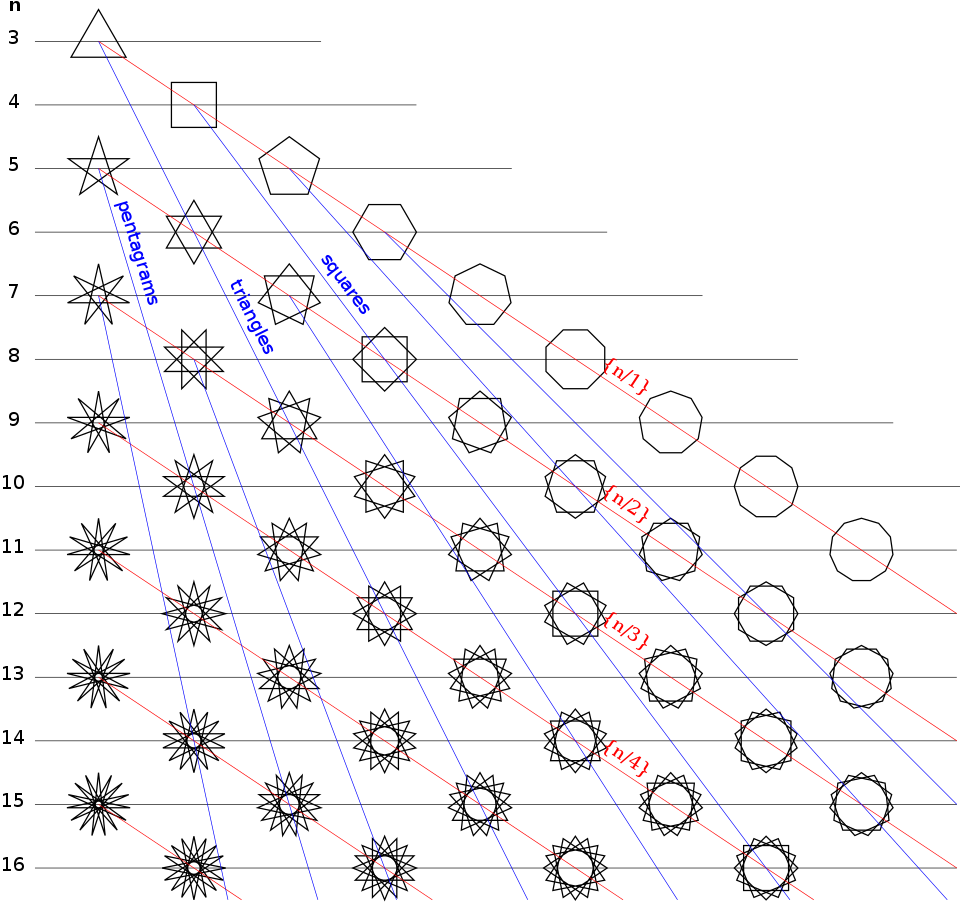
\includegraphics[width=0.8\textwidth]{images/polygons_1.png}
    \caption{A graph of the polygons}
\end{figure}
\begin{figure}[!htbp]
    \centering
    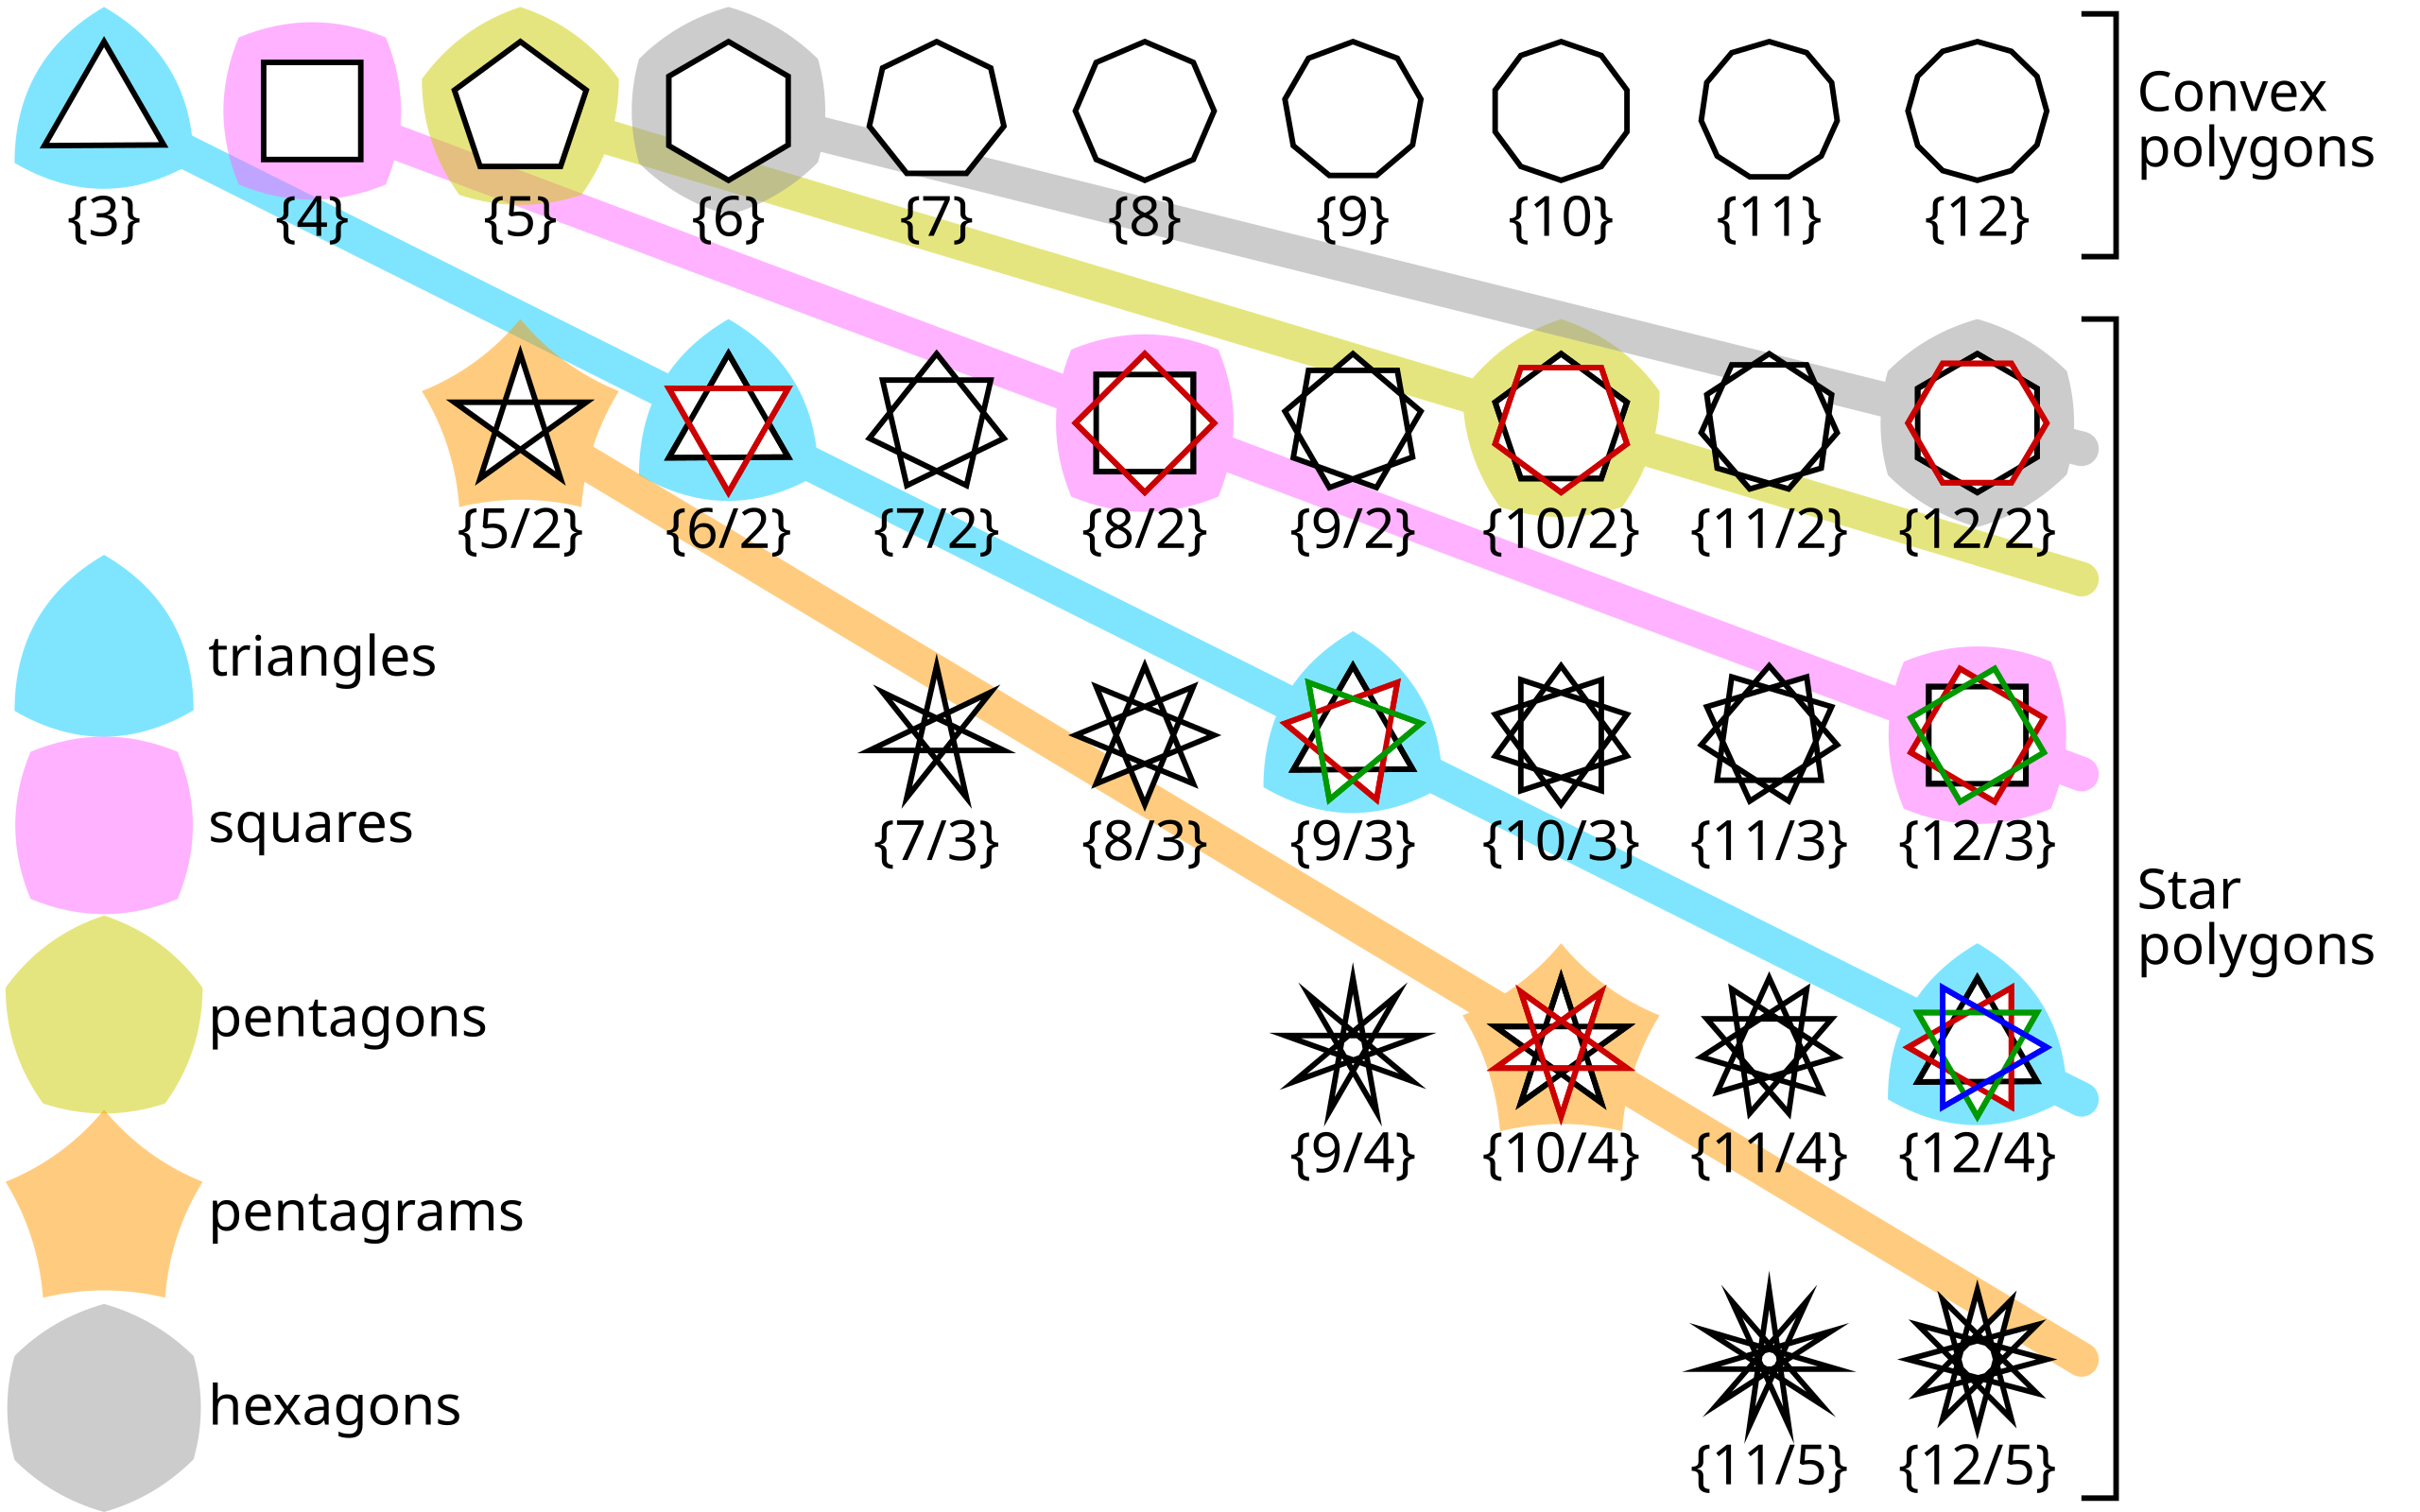
\includegraphics[width=0.8\textwidth]{images/polygons_2.png}
    \caption{A graph of the polygons}
\end{figure}


The Schläfli symbol is a recursive description, starting with $\{p\}$ for a $p$-sided regular polygon that is convex. For example, $\{3\}$ is an equilateral triangle, $\{4\}$ is a square, $\{5\}$ a convex regular pentagon, etc.

Regular star polygons are not convex, and their Schläfli symbols take the form $\{p/q\}$, where $p$ is the number of vertices and $q$ is their turning number. Equivalently, $\{p/q\}$ is created from the vertices of $\{p\}$ by connecting every $q$th vertex. For example, $\{5/2\}$ is a pentagram, while $\{5\}$ is a pentagon.

Note that $p$ and $q$ must be coprime, or the figure will degenerate, in which case we have the following theorem:

$\{p/q\}=d\{ \frac{p}{d} / \frac{q}{d} \}$, where $d=\gcd(p,q)$.

Let us define for any Schläfli symbol $\{p\} | n\{p\}$ for any $n$. It is intuitively true.

Then clearly axiom 1 is satisfied. Axiom 2 is also satisfied.

\subsubsection{Propositional Logic}

There are 3 flavors of $*$ in Propositional Logic: $\wedge, \vee, \rightarrow$. 

And we define $\phi | \psi$ if $\phi$ appears in $\psi$, for any wff $\phi, \psi$.

Then clearly all 4 of the core siumatgwoon axioms are satisfied. 

\begin{enumerate}
\item Trivial that all $\phi | \phi$
\item Also trivial that for any $\phi, \psi$, either $\phi|\psi$ or $\phi\not|\psi$.
\item Trivial as well that for any $\phi,\psi | \phi * \psi$.
\item Also trivial that if $\phi | \psi$ and $\psi | \theta$ then $\phi | \theta$.
\end{enumerate}

Propositional Logic as a Siumatgwoon has multiple interesting properties: 

\begin{enumerate}
\item It is compositionally complete. 
\item It is also constitutionally complete. 
\item Is it a simple siumatgwoon? Are decompositions finite? Yes. Are decompositions unique? Yes, up to reordering. So yes, it's a simple siumatgwoon.


\end{enumerate}


Consider the old siumatgwoon axioms, and a new relation "synonym", represented by $\sim$, read as "is synonymous with". It satisfies the following axioms.

\subsection{Synonym Axioms}

\begin{axiom}[Reflexivity]\label{ax:syn-reflex}
S1. (reflexivity) for all $x\in S$, $x\sim x$.
\end{axiom}

\begin{axiom}[Symmetry]\label{ax:syn-sym}
S2. (symmetry) For all $a,b\in S$, if $a\sim b$ then $b\sim a$.
\end{axiom}

\begin{axiom}[Transitivity]\label{ax:syn-trans}
S3. (transitivity) for all $a,b,c \in S$, if $a\sim b$, and $b \sim c$, then $a \sim c$.
\end{axiom}

\begin{axiom}[Compositional Congruence]\label{ax:syn-comp}
S4. (Compositional congruence) If $a \sim a'$, then (if they $ax$ or $xa$ exists):
\begin{itemize}
\item $ax \sim a'x$,
\item $xa \sim xa'$
\end{itemize}
\end{axiom}

\begin{axiom}[Composition Cancellation]\label{ax:syn-cancel}
S5. Composition cancellation
\begin{itemize}
\item If $a * b \sim a * c$, then $b \sim c$;
\item If $b*a\sim c*a$ then $b \sim c$;
\end{itemize}
\end{axiom}

\begin{axiom}[Divisor Compatibility]\label{ax:syn-div}
S6. Divisor compatibility: If $a \sim b$, then for all $x \in S$, $x|a$ iff $x|b$.
\end{axiom}

\begin{axiom}[Upwards Divisibility]\label{ax:syn-up}
S7: Upwards divisibility: If $a\sim b$, then for all if $a|x$ then $b|x$.
\end{axiom}

A Siumatgwoon is Synonym-Closed if in which if $a*b$ exists and $a\sim a'$ and $b\sim b'$ then $a'*b, a*b', a'*b'$ also exist. Most siumatgwoons, including the Sinoglyphs, are not synonym-closed. 

Because of S4, Synonym-Closed Siumatgwoons must have $a*b \sim a'*b \sim a*b'\sim a'*b'$.

\subsection{S8: Synonym Replacement and Existence Preservation}

Synonym replacement completion: if $a*b$ exists, and if $b\sim b'$, then $a*b'$ exists in $S$ as well.

Prior to this, we are rather ambiguous and coy as to whether $a$ and $b$ being synonymous means $b*x$ necessarily exists if $a*x$ exists. I feel we should admit closure for synonym substitutional compositions. We can consider other structure where this axiom is not admitted later.

S9. Multidecomposition if $ab \sim cd$ and $cd = e$ then $ab =e$. 

From S4 you'd be able to prove that $a \sim a'$ and $b\sim b'$ then $a * b \sim a' * b'$.

\section{The Quotient Siumatgwoon $S/\sim$}

\subsection{Starting Point: Synonymy $\sim$ as an Equivalence Relation}

Let $S$ be a Siumatgwoon, and let $\sim$ be a synonymy relation on $S$ satisfying:

\begin{itemize}
\item $\sim$ is an equivalence relation: reflexive, symmetric, transitive.
\item $\sim$ is \textbf{compatible with composition}:
    
    If $a\sim a'$, $b\sim b'$, then $a*b\sim a'*b'$.
    
\item $\sim$ is \textbf{compatible with divisibility}:
    
    If $a\sim b$, then $x|a \iff x|b$ for all $x\in S$.
\end{itemize}

These give us a solid foundation to define a quotient structure.

\subsection{The Set $S/\sim$}

Let:

$S/\sim=\{[a]:a\in S\}$

where $[a]=\{x\in S\mid x\sim a\}$ is the \textbf{equivalence class} of $a$.

\subsection{Defining the Operations on $S/\sim$}

\subsubsection{Multiplication}

We define:

$[a]*[b]:=[a*b]$, if $a*b$ exists.

This is well-defined \textbf{because of compositional congruence} (axiom S4).

It is also because that we required if $a*b$ exists, so must $a'*b'$.

That is: if $a \sim a'$, and $b \sim b'$, then:

$a*b\sim a'*b'\Rightarrow [a*b]=[a'*b']$

So the result is independent of the representative.

\subsubsection{Divisibility}

We define:

$[a]|[b] \iff a|b$

Again, this is \textbf{well-defined} thanks to the \textbf{divisibility equivalence} axiom (S6):

If $a\sim a', b \sim b'$, given we have the axiom that $a|b \iff a'|b'$ then:

$[a]|[b] \iff [a']|[b']$

Thus, $|$ descends to the quotient.

\subsection{Verifying Siumatgwoon Axioms in $S/\sim$}

Let's verify that the \textbf{quotient structure inherits} the original Siumatgwoon axioms:

\begin{itemize}
\item \textbf{Axiom 1 (Reflexivity of $|$)}:
    
    Since $a|a\Rightarrow[a]|[a]$
    
\item \textbf{Axiom 2 (Totality)}:
    
    For all $[a],[b]$, either $[a]|[b]$ or not.
    
    This follows since $|$ on $S$ has totality, and divisibility is preserved under $\sim$.
    
\item \textbf{Axiom 3 (Transitivity)}:
    
    Suppose $[a]|[b]$ and $[b]|[c]$. Recall the definition that $[a]|[b]$ then $a|b$. It's straightforward.
    
\item \textbf{Axiom 4 (Composition and divisibility)}:
    
    We want to prove that if $[a]*[b]=[c]$, then $[a],[b] | [c]$. By definition $[a]*[b]=[c]$ then $a*b\sim c$, and so $a|c$. By the definition of constitutiveness over synonym classes, $[a]|[c]$. The argument same goes for $[b]|[c]$.
\end{itemize}

Now come axioms 5 and axioms 6. Do they hold in $S/\sim$, even if they might not hold in $S$?

\begin{itemize}
\item Axiom 5 (Complete Constructibility and Generators): There exists a non-empty subset $G_{S} \subseteq S$ such that:
    \begin{itemize}
    \item (Generation) Every element $x \in S$ is a product of a finite sequence of elements from $G_S$, i.e., $x = g_1 * g_2 * \cdots * g_n$, where $g_1, \dots, g_n \in G_S$
    \end{itemize}

And a Simple Siumatgwoon is one where:

\begin{enumerate}
\item $E$ is a generating set, and 
\item that decompositions into elementals are unique.
\end{enumerate}

\item Axiom 6. (Finite constitution). For any $x \in S$, there are only finitely many objects $y_1, y_2, \ldots, y_n \in S$ such that $y_1, y_2, \ldots, y_n | x$.
\end{itemize}

Let's prove that axiom 5 holds first. And then axiom 6 holds. Then we prove that $S/\sim$ is a simple siumatgwoon.

Consider some element $[x] \in S/\sim$. Given $S$ is a siumatgwoon, we know that any $x$ has a finite decomposition $g_1 * g_2 * g_3 * \cdots g_n$. Given $x=g_1 * g_2 * g_3 * \cdots g_n$, we have $[x]=[g_1 * g_2 * g_3 * \cdots g_n]$, and by the definition of $[*]$ we have $[x]=[g_1 * g_2 * g_3 * \cdots g_n]=[g_1] * [g_2] * [g_3] * \cdots [g_n]$. Given this applies to every $x$ in $S$, it is true of every $[x]\in S/\sim$. 

Note that some of the $[g_i]$ might be equal to some other $[g_j]$ if $g_i \sim g_j$.

Now for axiom 6.

Consider $[x]\in S/\sim$. By axiom 6, there only finitely many $y_1, y_2, \ldots, y_n | x.$ Therefore there are only finitely many $[y_1], [y_2], \ldots, [y_n] | [x].$ Note again, that because there could be $y_i \sim y_j$, then the most reduced list of constituents for $[x]$ might be shorter than $n$.

\textbf{Axiom 5 (Generators)}:

If $G\subseteq S$ is a generating set, then $[G]=\{[g]\mid g\in G\}\subseteq S/\sim$ generates all of $S/\sim$

Hence, $S/\sim$ is a well-defined \textbf{quotient Siumatgwoon}.

\subsection{Interpretation of $S/\sim$}

\begin{itemize}
\item \textbf{Elements of $S/\sim$} are \textbf{semantic classes}: bundles of expressions that mean the same thing.
\item \textbf{Operations and structure} are all inherited from how the parts combine.
\item This is essentially a move from \textbf{syntax to semantics} — a form of canonical simplification.
\end{itemize}

\subsection{Identity and Atoms in $S/\sim$}

\begin{itemize}
\item The set of \textbf{atomic classes} would be:

$A/\sim=\{[a]\mid a\in A\}$

If synonymy is strong (e.g., if all synonyms of atoms are equal), then this is a \textbf{true set of atomic meanings}.

\item The quotient set \textbf{removes redundancy}: if two characters are written differently but function identically, they're collapsed.
\end{itemize}

\section{A Hierarchy of Synonym Relations}

Intuitively speaking, the $\sim$ of 言$\sim$文 that allows us write 信$\sim$伩 seems different from the $\sim$ in 女$\sim$巫, as it does not seem the case that 女 can be exchanged for 巫 in all Chinese characters. This suggests that there is a hierarchy, or rather, a family of synonymous relations, perhaps context dependent. 

Some synonyms are more closely clustered together than others. This suggests there is a hierarchy of synonyms.



But to interpret $~$ to only mean "is synonymous with", leaves us certain phenonomena in, or rather, certain ways to "play" Chinese characters, uncaptured. 

In Classical Chinese poetry and prose, it is appreciated if couplets are written in a way that characters in the same position belong to "some same class" or objects. 

Consider all these lines from 《增廣賢文》:


兩人一般心,無錢堪買金;一人一般心,有錢難買針。
馬行無力皆因瘦,人不風流只爲貧。

畫虎畫皮難畫骨,知人知面不知心。
錢財如糞土,仁義値千金。
流水下灘非有意,白雲出岫本無心。

路遙知馬力,日久見人心。
相見易得好,久住難爲人。
饒人不是癡漢,癡漢不會饒人。
有錢道眞語,無錢語不眞。
長江後浪推前浪,世上新人趕舊人。
來如風雨,去似微塵。
萬般皆是命,半點不由人。


寧可正而不足,不可邪而有餘。
寧可信其有,不可信其無。


To illustrate the point, consider this following sentence, taken from the Analects. 

萬方有罪,罪在朕躬。

"Whoever is sinful, the guilt is on my body."

This sentence clearly expresses a monarchist position of politics - one that is shared by both classical Confucianism and medieval Christian political theory. The sovereign, the 君主, is the one who bears the responsibility, and the sins of the 萬方.

Let us simplify and modify this sentence a bit: 

君主之國,萬方有罪,罪在君身。

"In a country where monarchs are sovereign, whoever is sinful, the guilt is on the monarch's body."

Now a we can apply a naive application of lax synonymy, say on 萬 ("ten thousand") and 兆 ("trillion"), drawing upon they can both be taken to mean "uncountably many" on a metaphoric level, so $\text{萬} \sim \text{兆}$, so we get 
$$
\text{君主之國,\underline{萬}方有罪,罪在君身}
\sim
\text{君主之國,\underline{兆}方有罪,罪在君身}
$$

We don't have the full algebraic machinery to justify this yet, but it is reasonable. 

What I really want to point out, is that in a sense, 君 and 民 belong to the same class - the same class of objects, political objects that is, that can occupy the position of 君. So in a sense, we can write $\text{君} \sim_{?} \text{民}$. Then, by simply substituting 君 for 民, we get 

$$
\text{\underline{民}主之國,萬方有罪,罪在\underline{君}身} \sim_{?} \text{\underline{民}主之國,兆方有罪,罪在\underline{民}身}
$$

Which says, "in a country where the people are sovereign, whoever is sinful, the guilt is on the people's body." 



This is not a derivation. Or is it? What kind of derivation is this? What kind of rule of inference are we appealing to? And what is the argument sayiing? Are we saying if (君主之國,萬方有罪,罪在朕躬) and $\text{君} \sim_{?} \text{民}$ then we can derive (民主之國,萬方有罪,罪在民身)? What laws govern the behaviour of the $\sim_{?}$? Are they the same as the laws governing the behaviour of $\sim$?



\end{document}
